% !TEX root = _main.tex

\section{楽曲データベース}
\label{app:database}
本研究で使用した楽曲データベースの詳細を示す．


\begin{figure*}[tb]
	\centering
	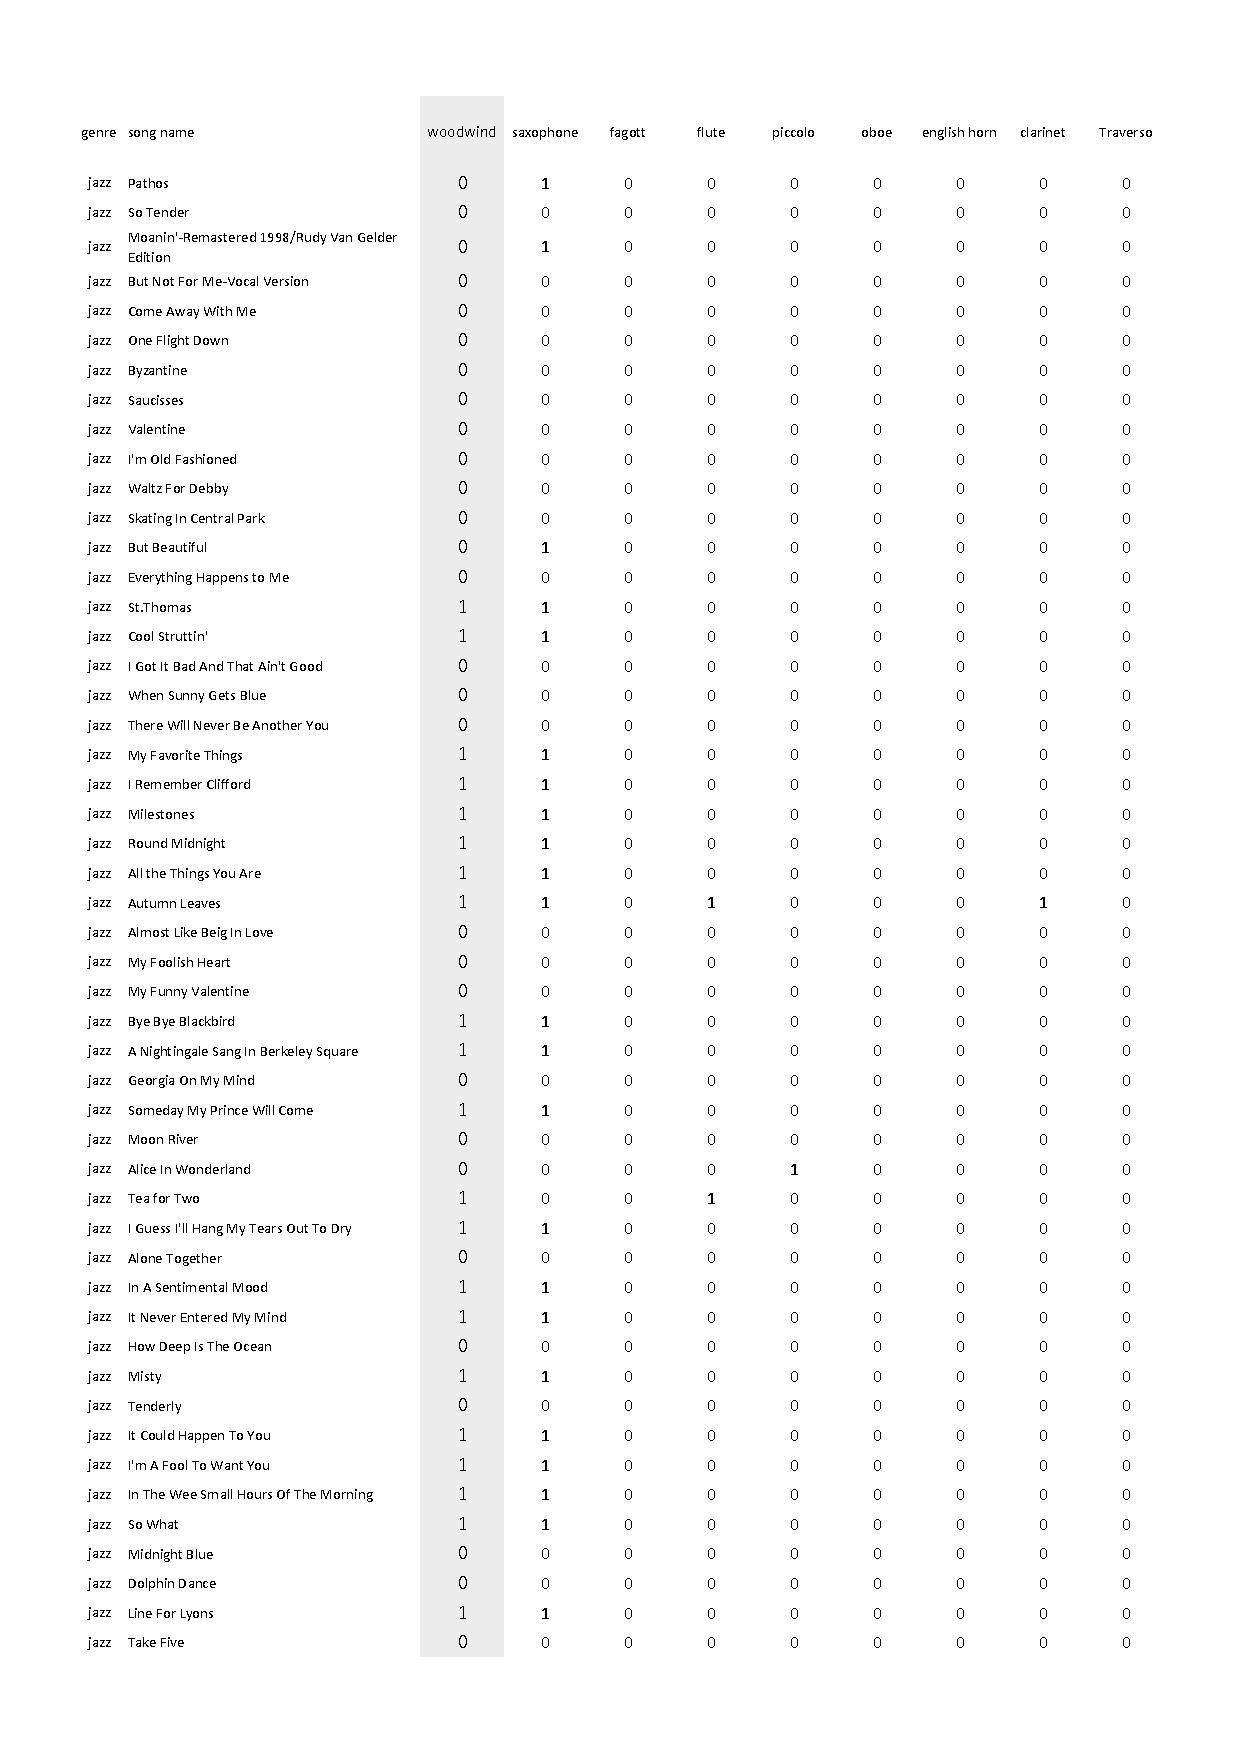
\includegraphics[width=.8\hsize]{fig/fig37-testdata1.pdf}
	\label{fig:1}
\end{figure*}

\begin{figure*}[tb]
	\centering
	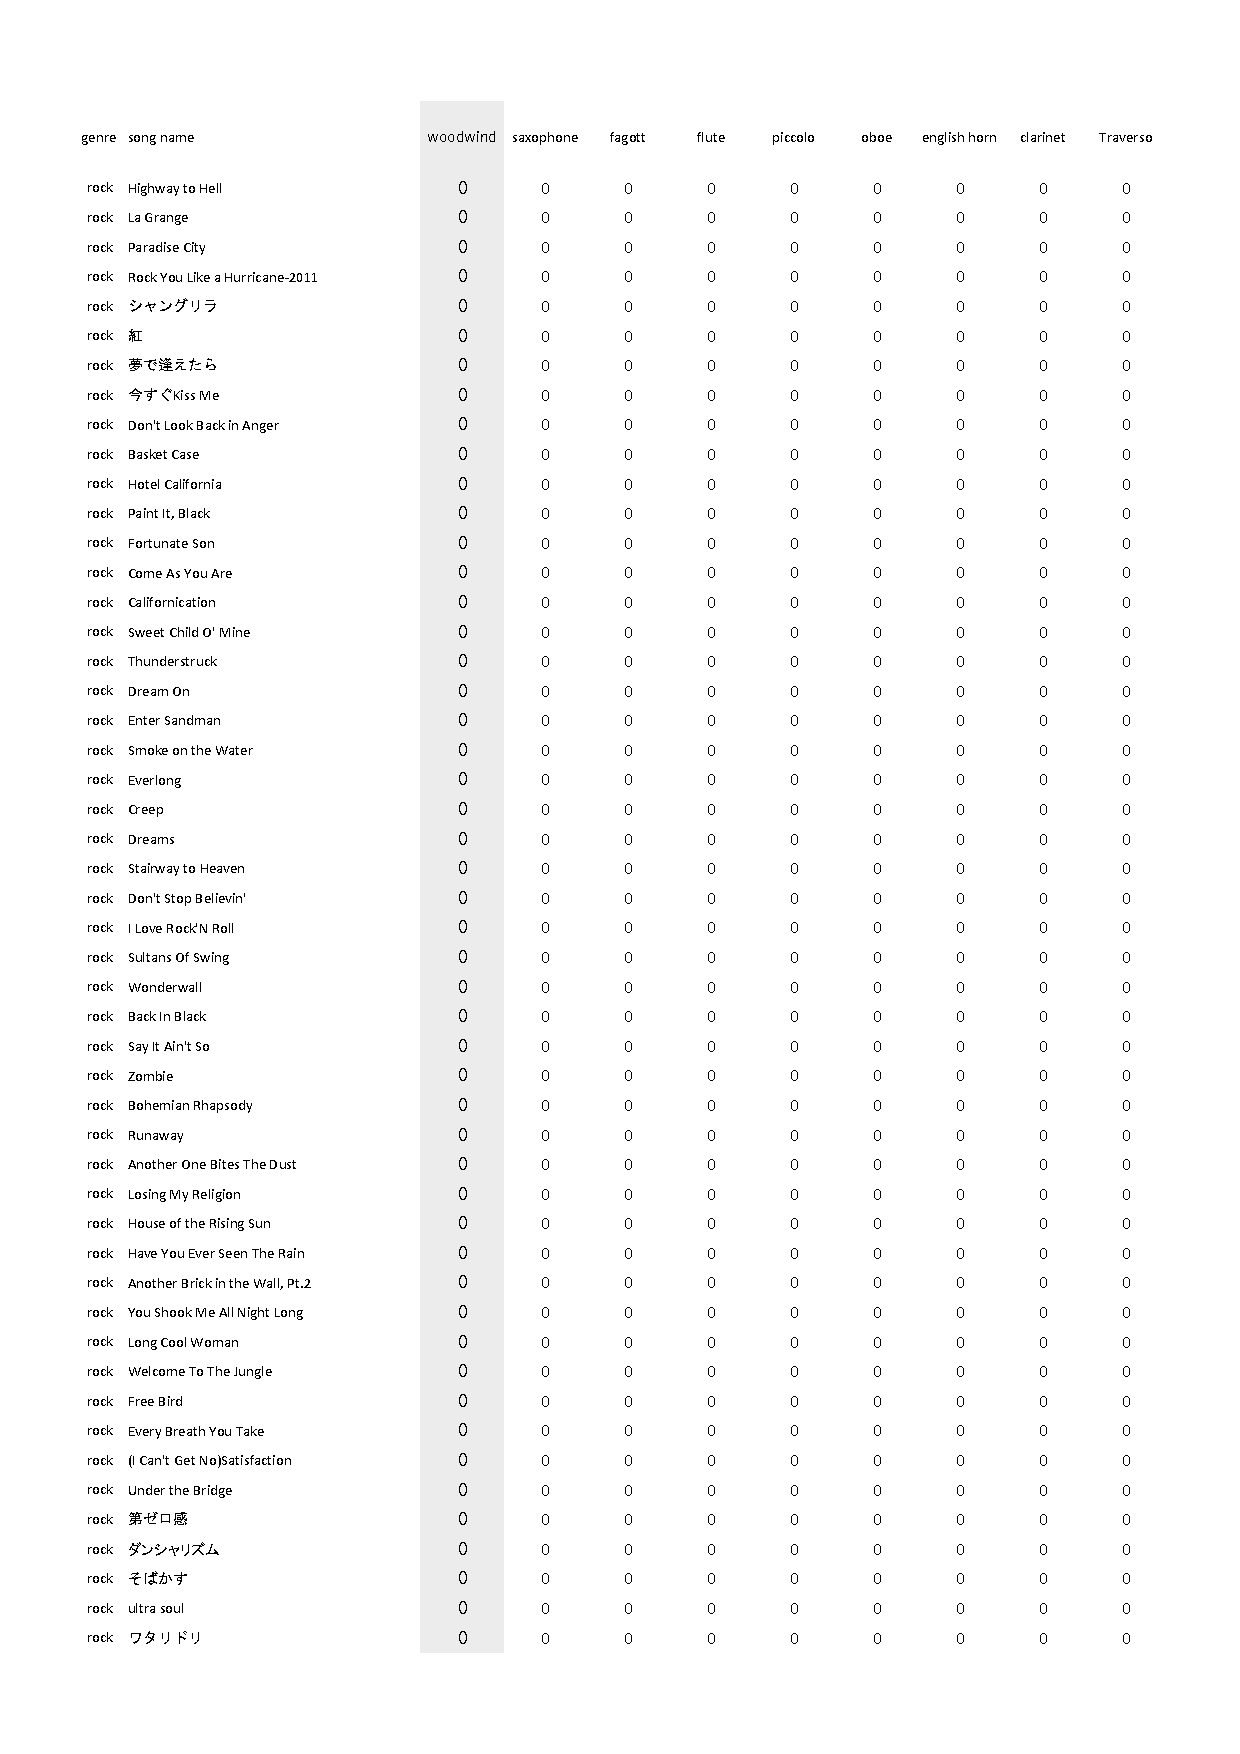
\includegraphics[width=.8\hsize]{fig/fig38-testdata2.pdf}
	\label{fig:2}
\end{figure*}

\begin{figure*}[tb]
	\centering
	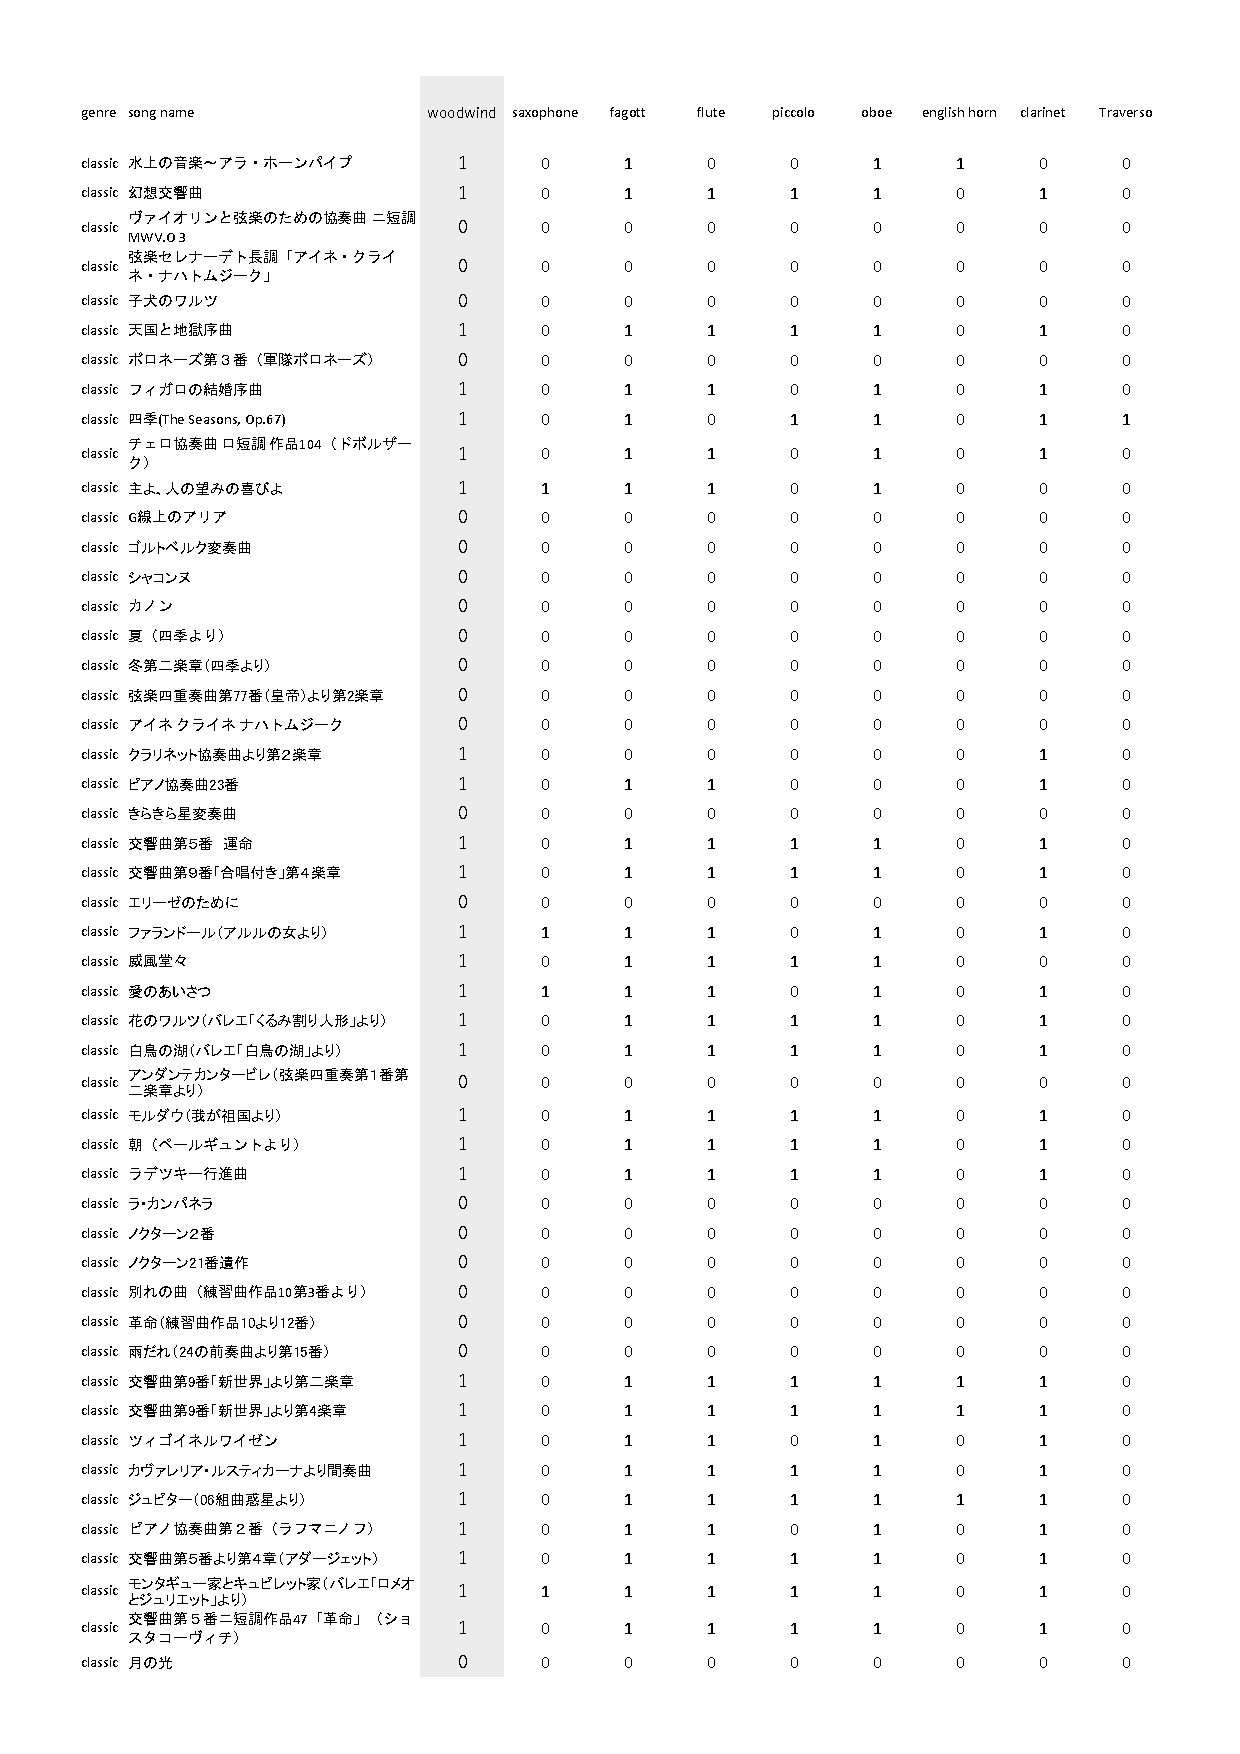
\includegraphics[width=.8\hsize]{fig/fig39-testdata3.pdf}
	\label{fig:3}
\end{figure*}

\begin{figure*}[tb]
	\centering
	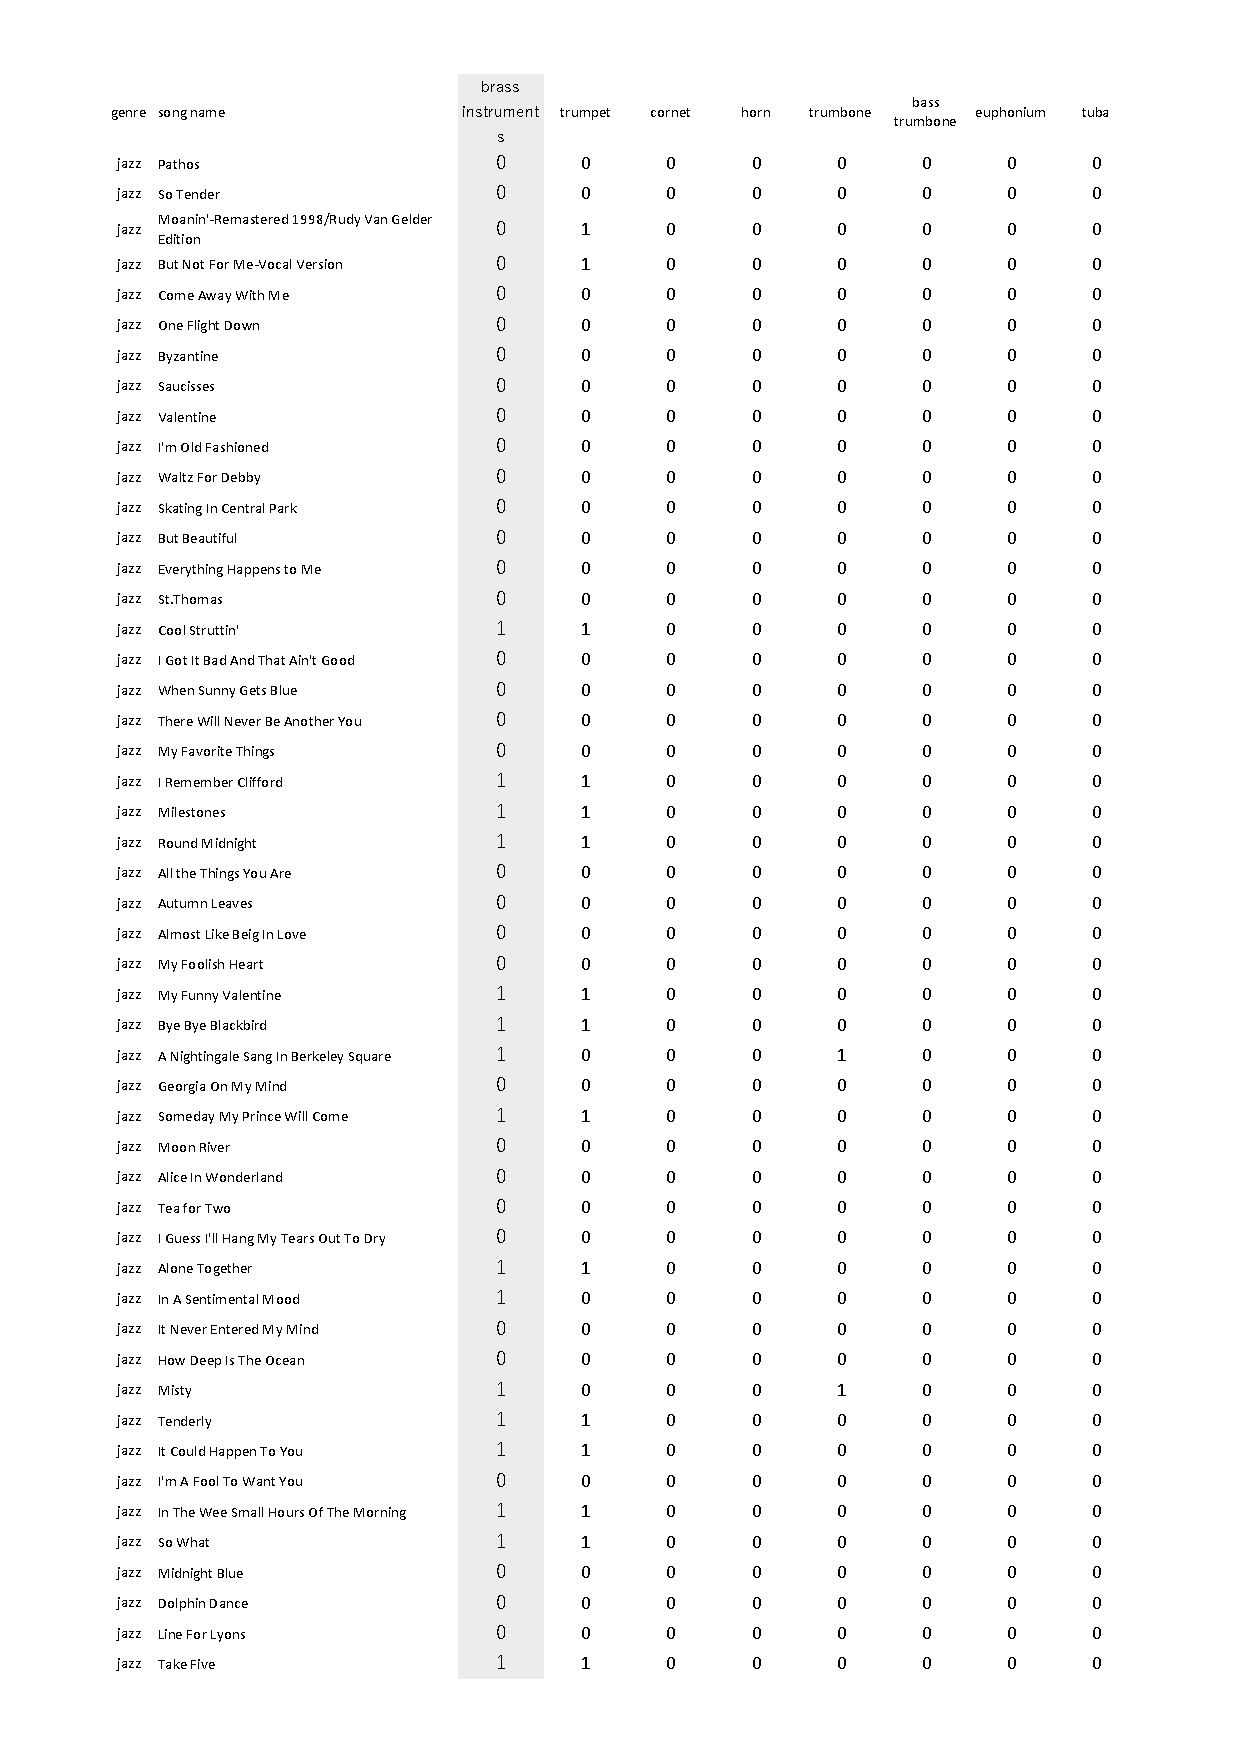
\includegraphics[width=.8\hsize]{fig/fig40-testdata4.pdf}
	\label{fig:4}
\end{figure*}

\begin{figure*}[tb]
	\centering
	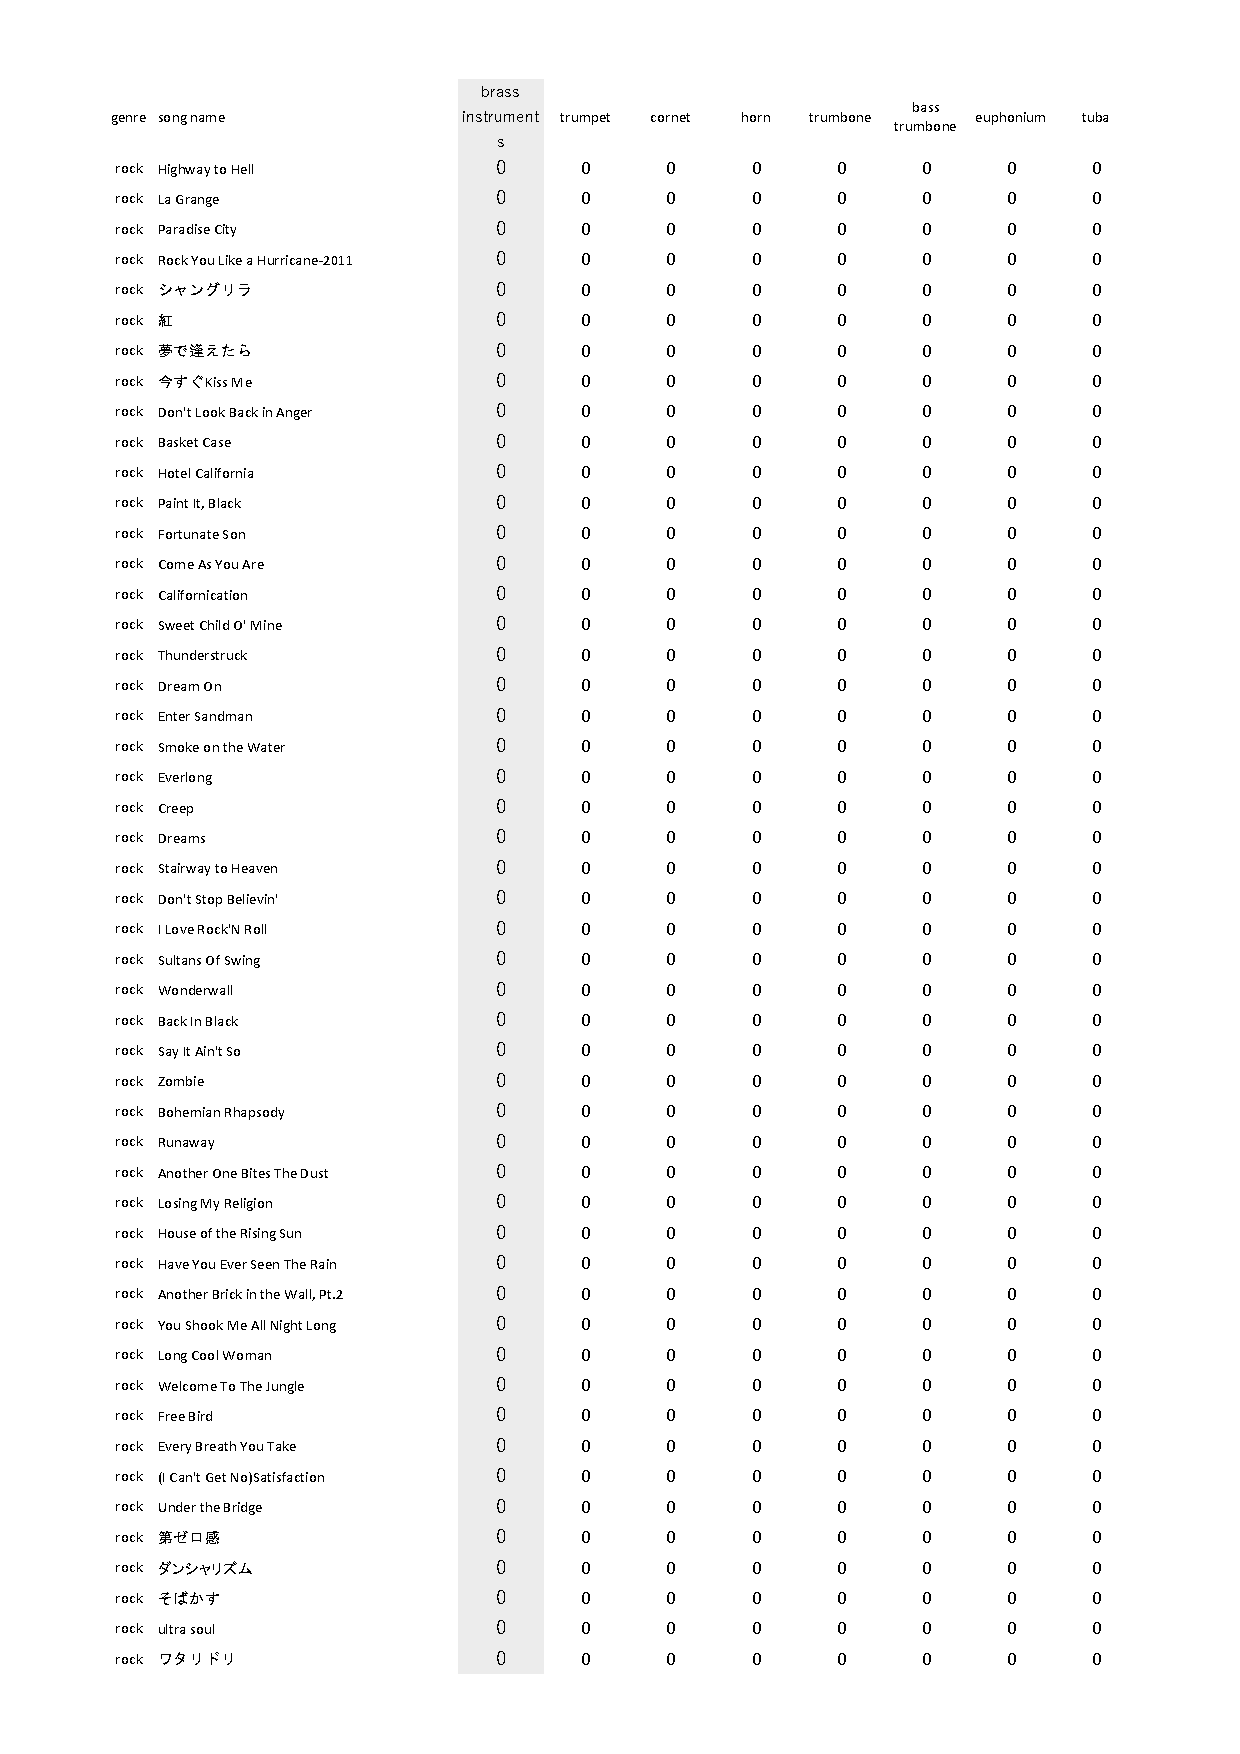
\includegraphics[width=.8\hsize]{fig/fig41-testdata5.pdf}
	\label{fig:5}
\end{figure*}

\begin{figure*}[tb]
	\centering
	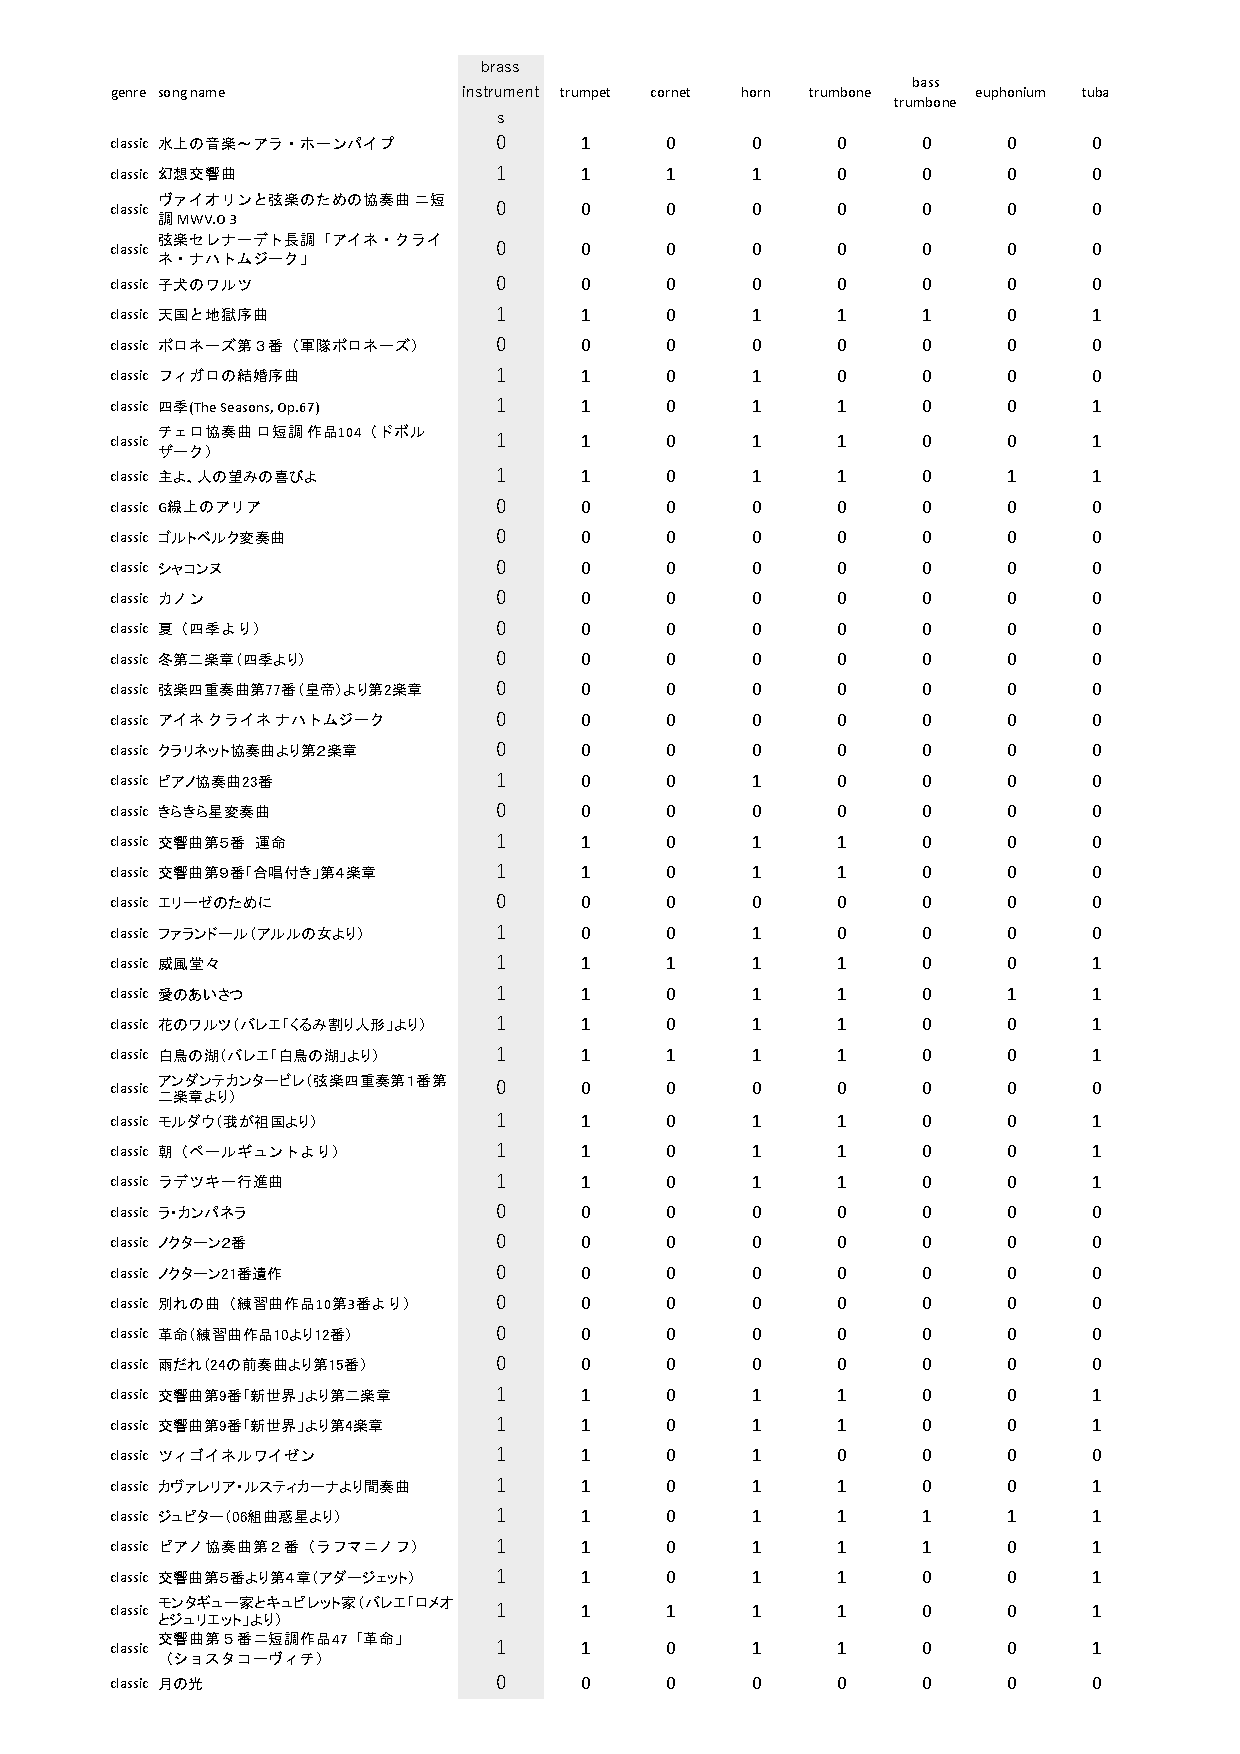
\includegraphics[width=.8\hsize]{fig/fig42-testdata6.pdf}
	\label{fig:6}
\end{figure*}

\begin{figure*}[tb]
	\centering
	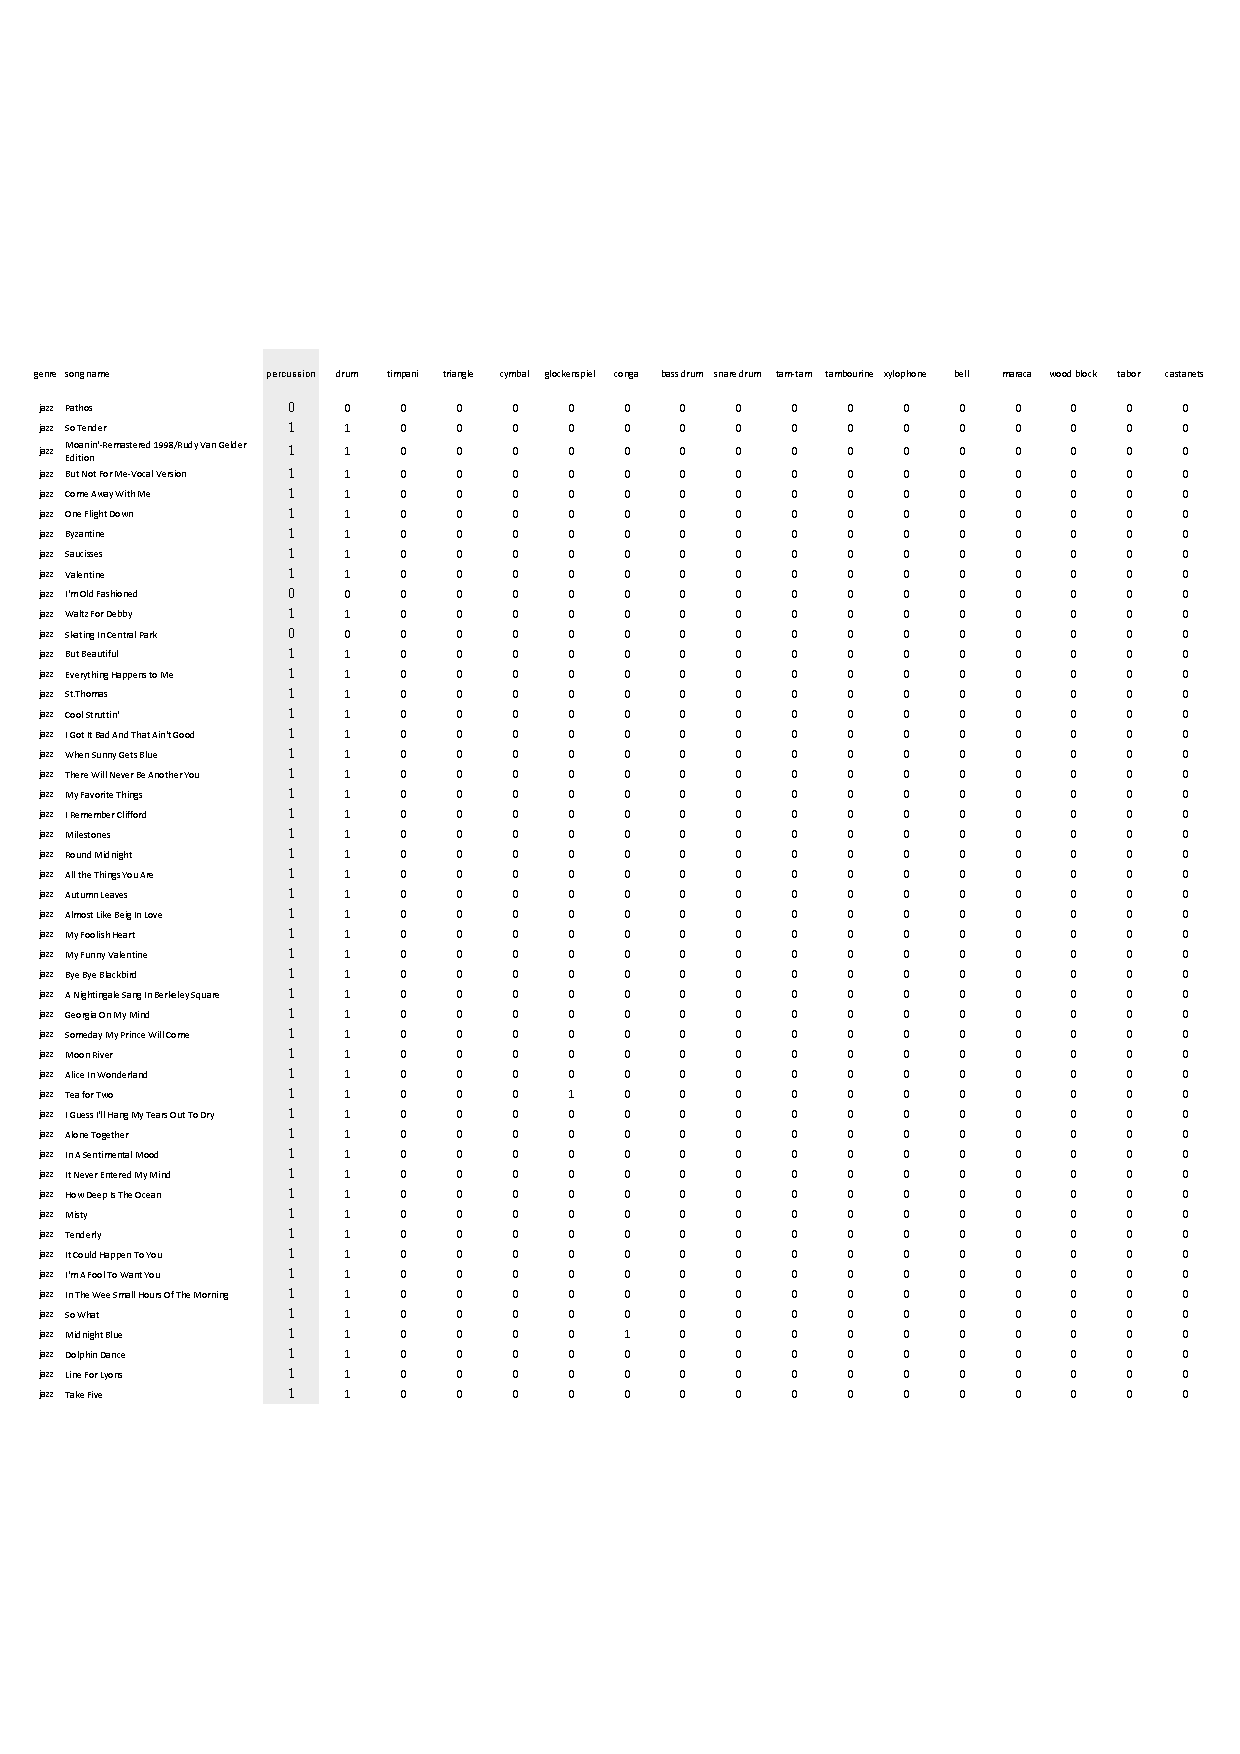
\includegraphics[width=.8\hsize]{fig/fig43-testdata7.pdf}
	\label{fig:7}
\end{figure*}

\begin{figure*}[tb]
	\centering
	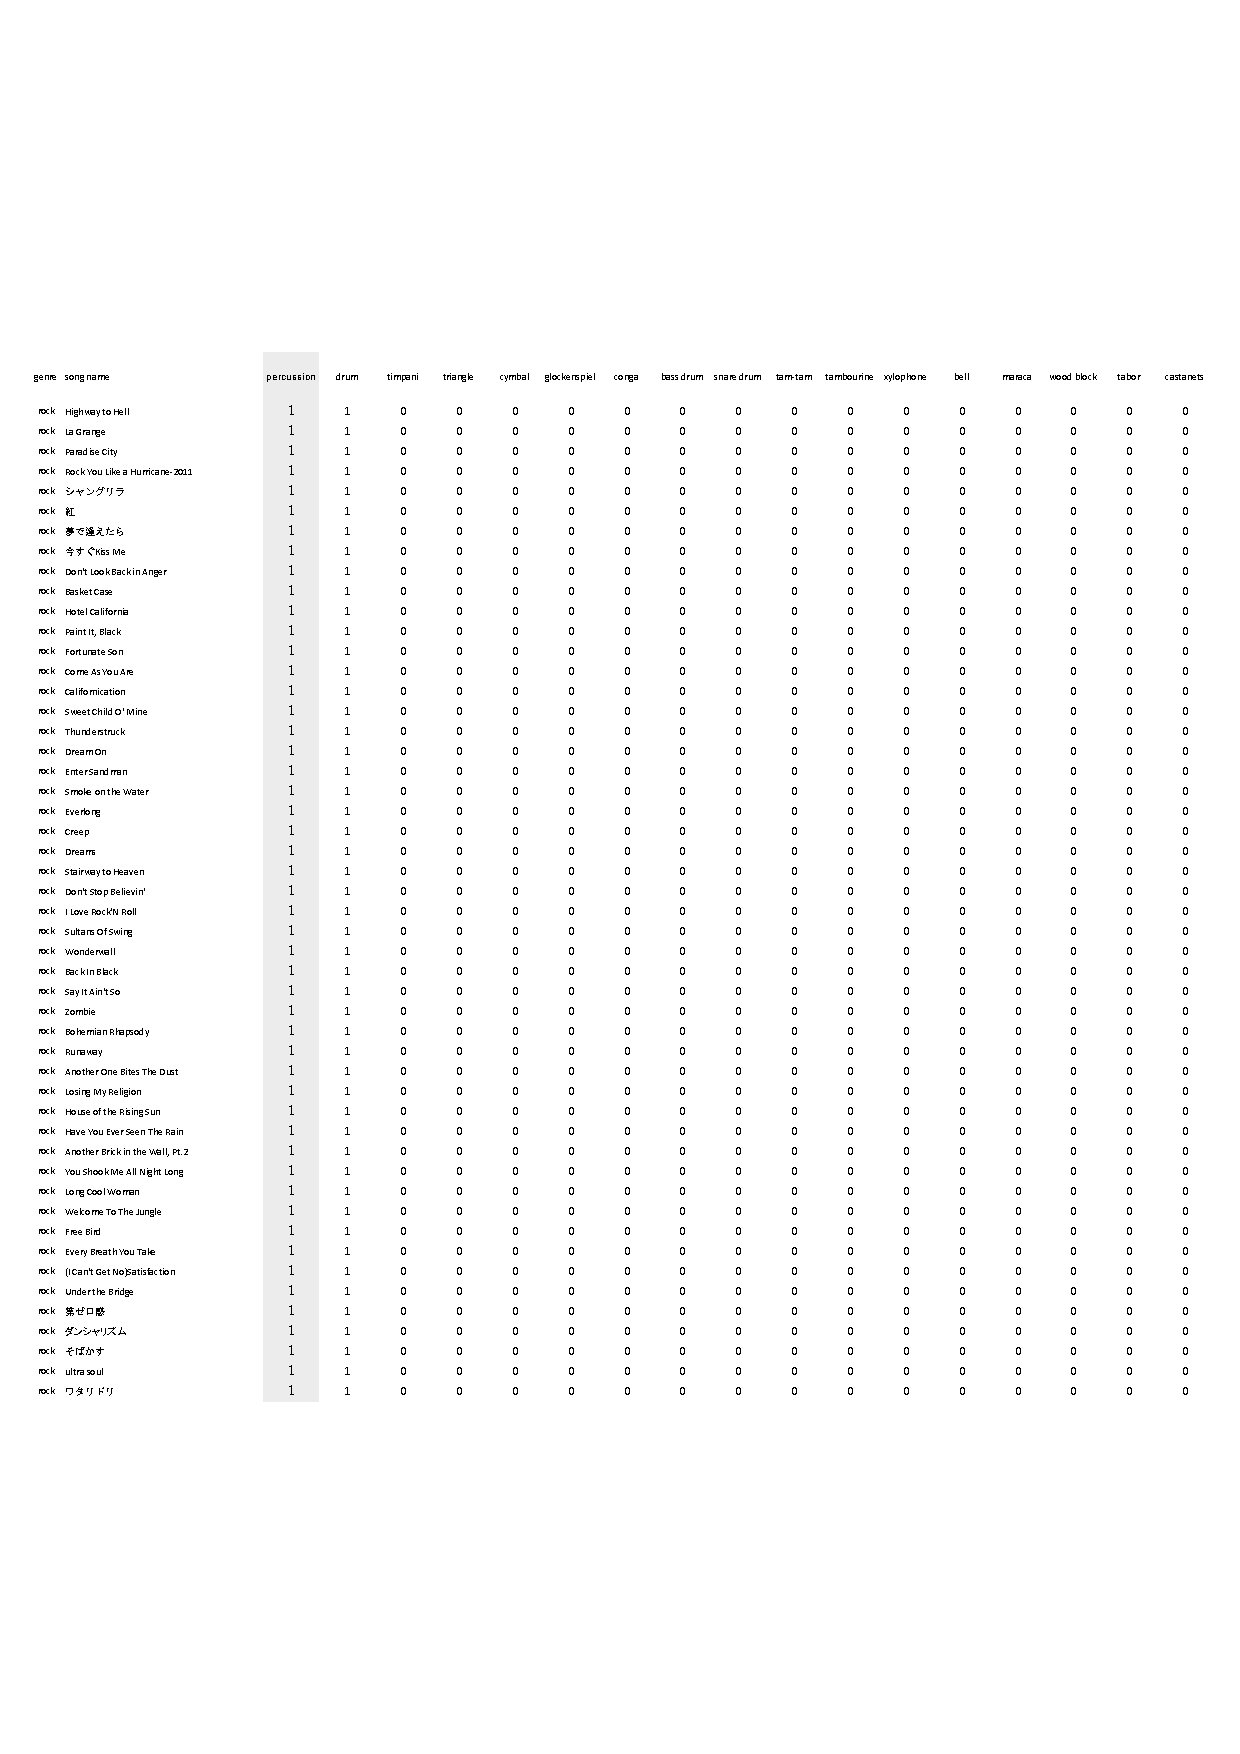
\includegraphics[width=.8\hsize]{fig/fig44-testdata8.pdf}
	\label{fig:8}
\end{figure*}

\begin{figure*}[tb]
	\centering
	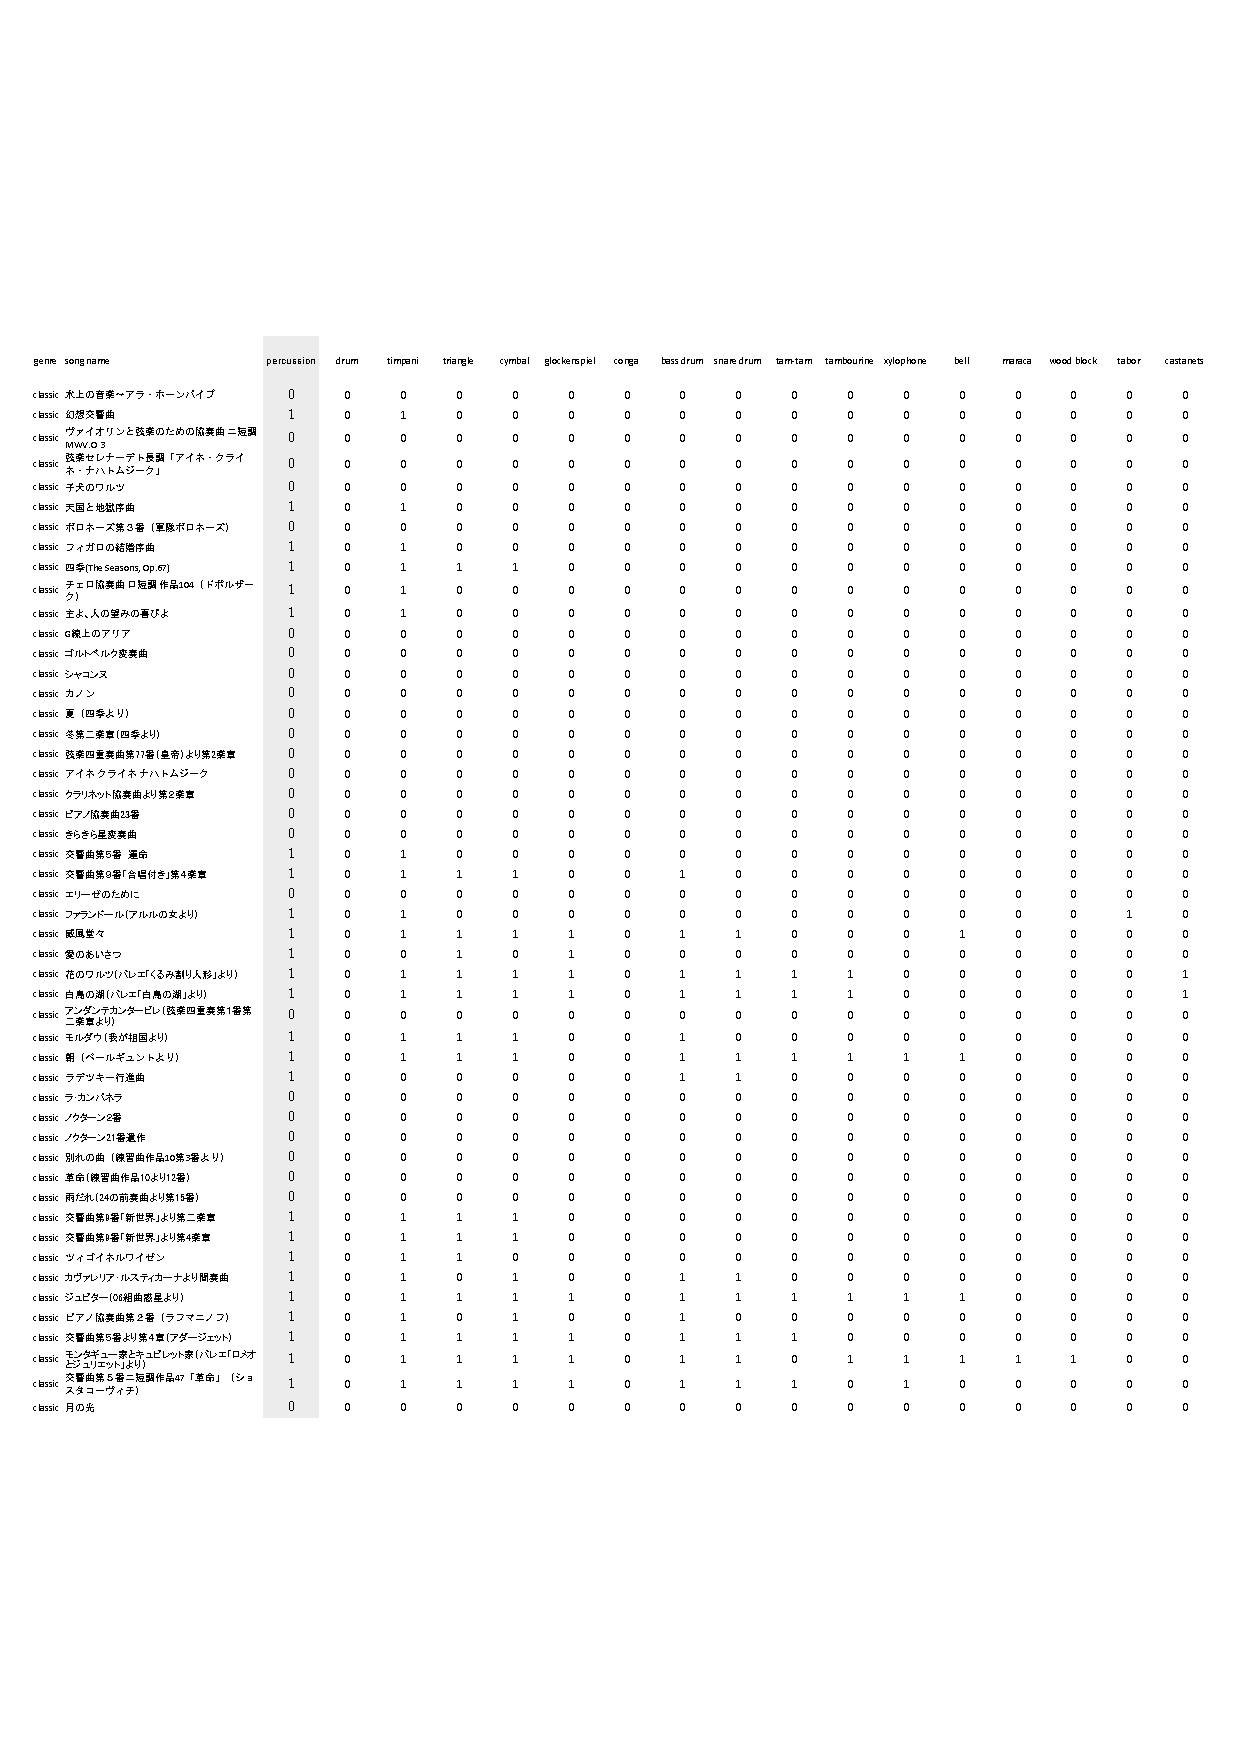
\includegraphics[width=.8\hsize]{fig/fig45-testdata9.pdf}
	\label{fig:9}
\end{figure*}

\begin{figure*}[tb]
	\centering
	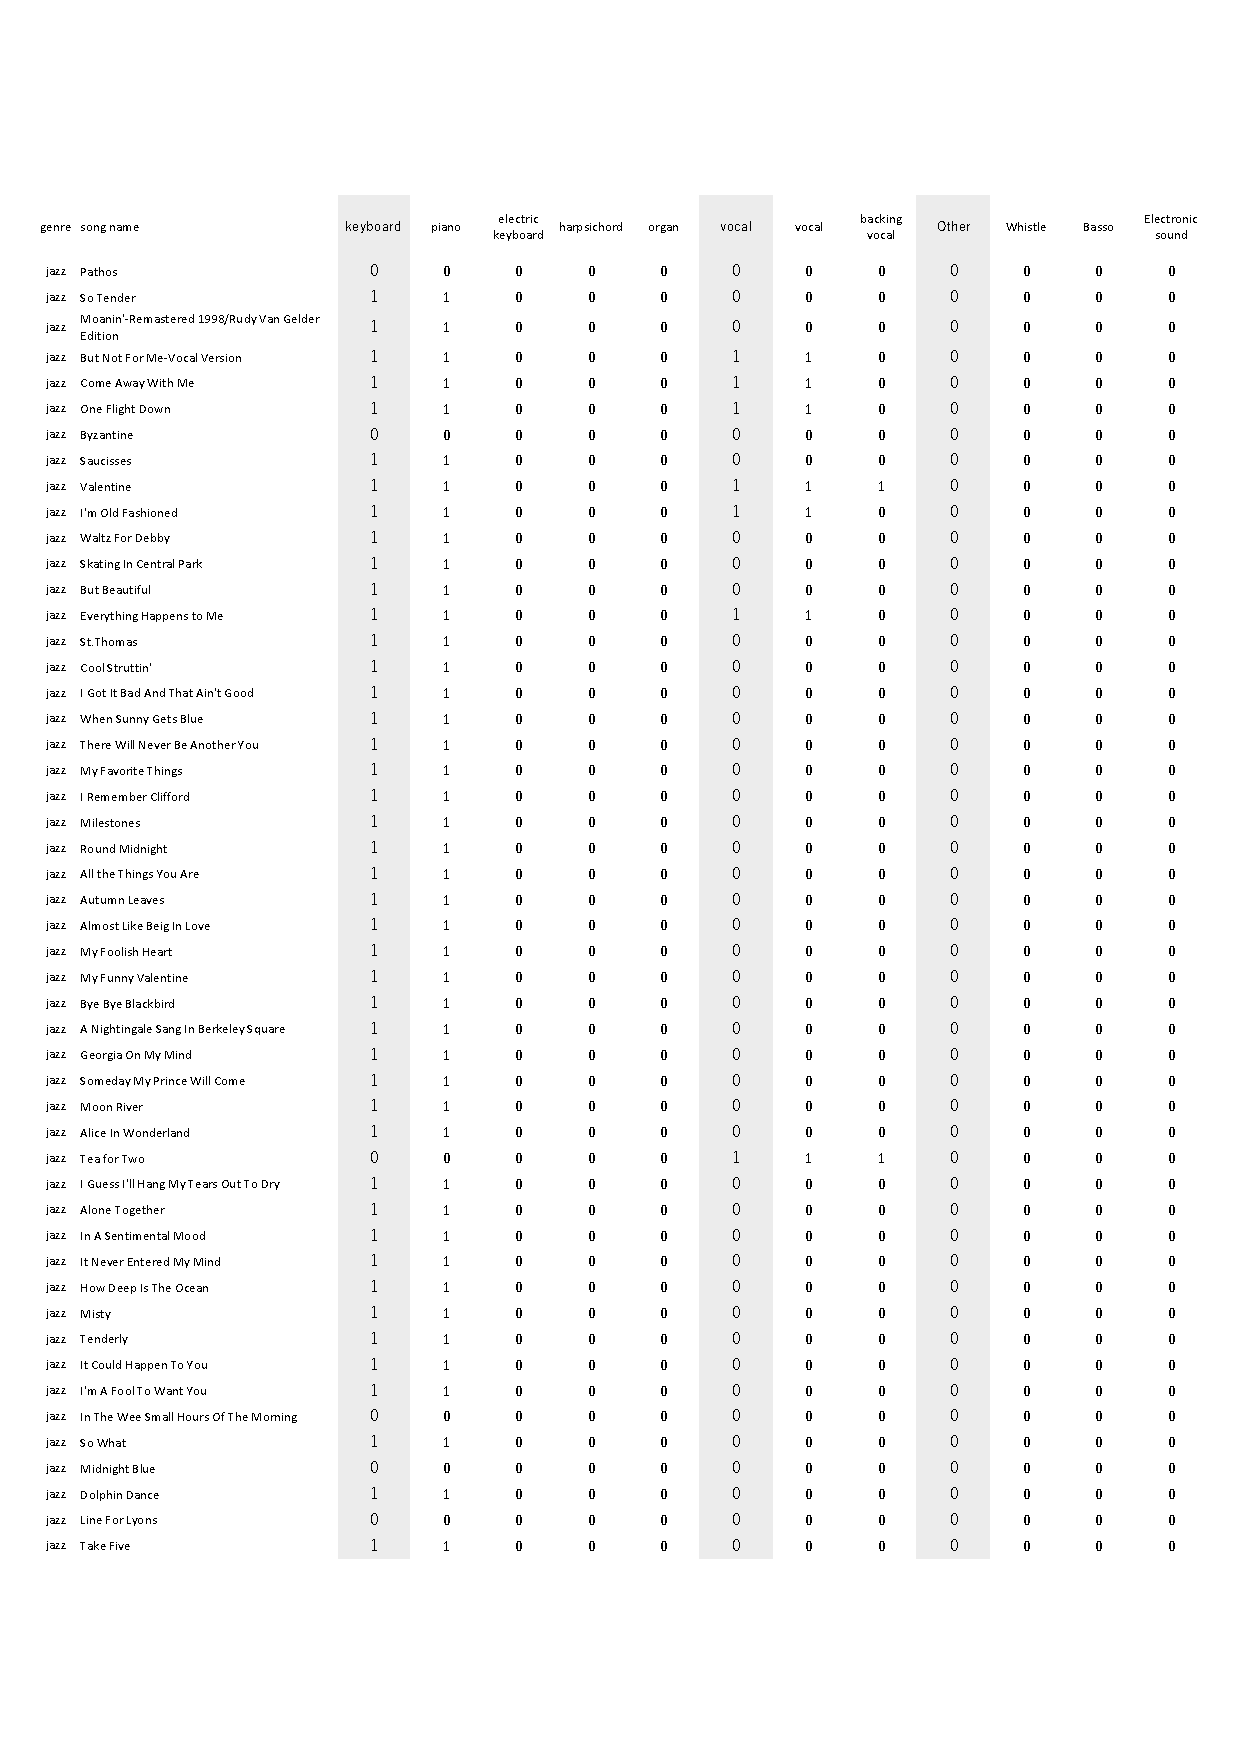
\includegraphics[width=.8\hsize]{fig/fig46-testdata10.pdf}
	\label{fig:10}
\end{figure*}

\begin{figure*}[tb]
	\centering
	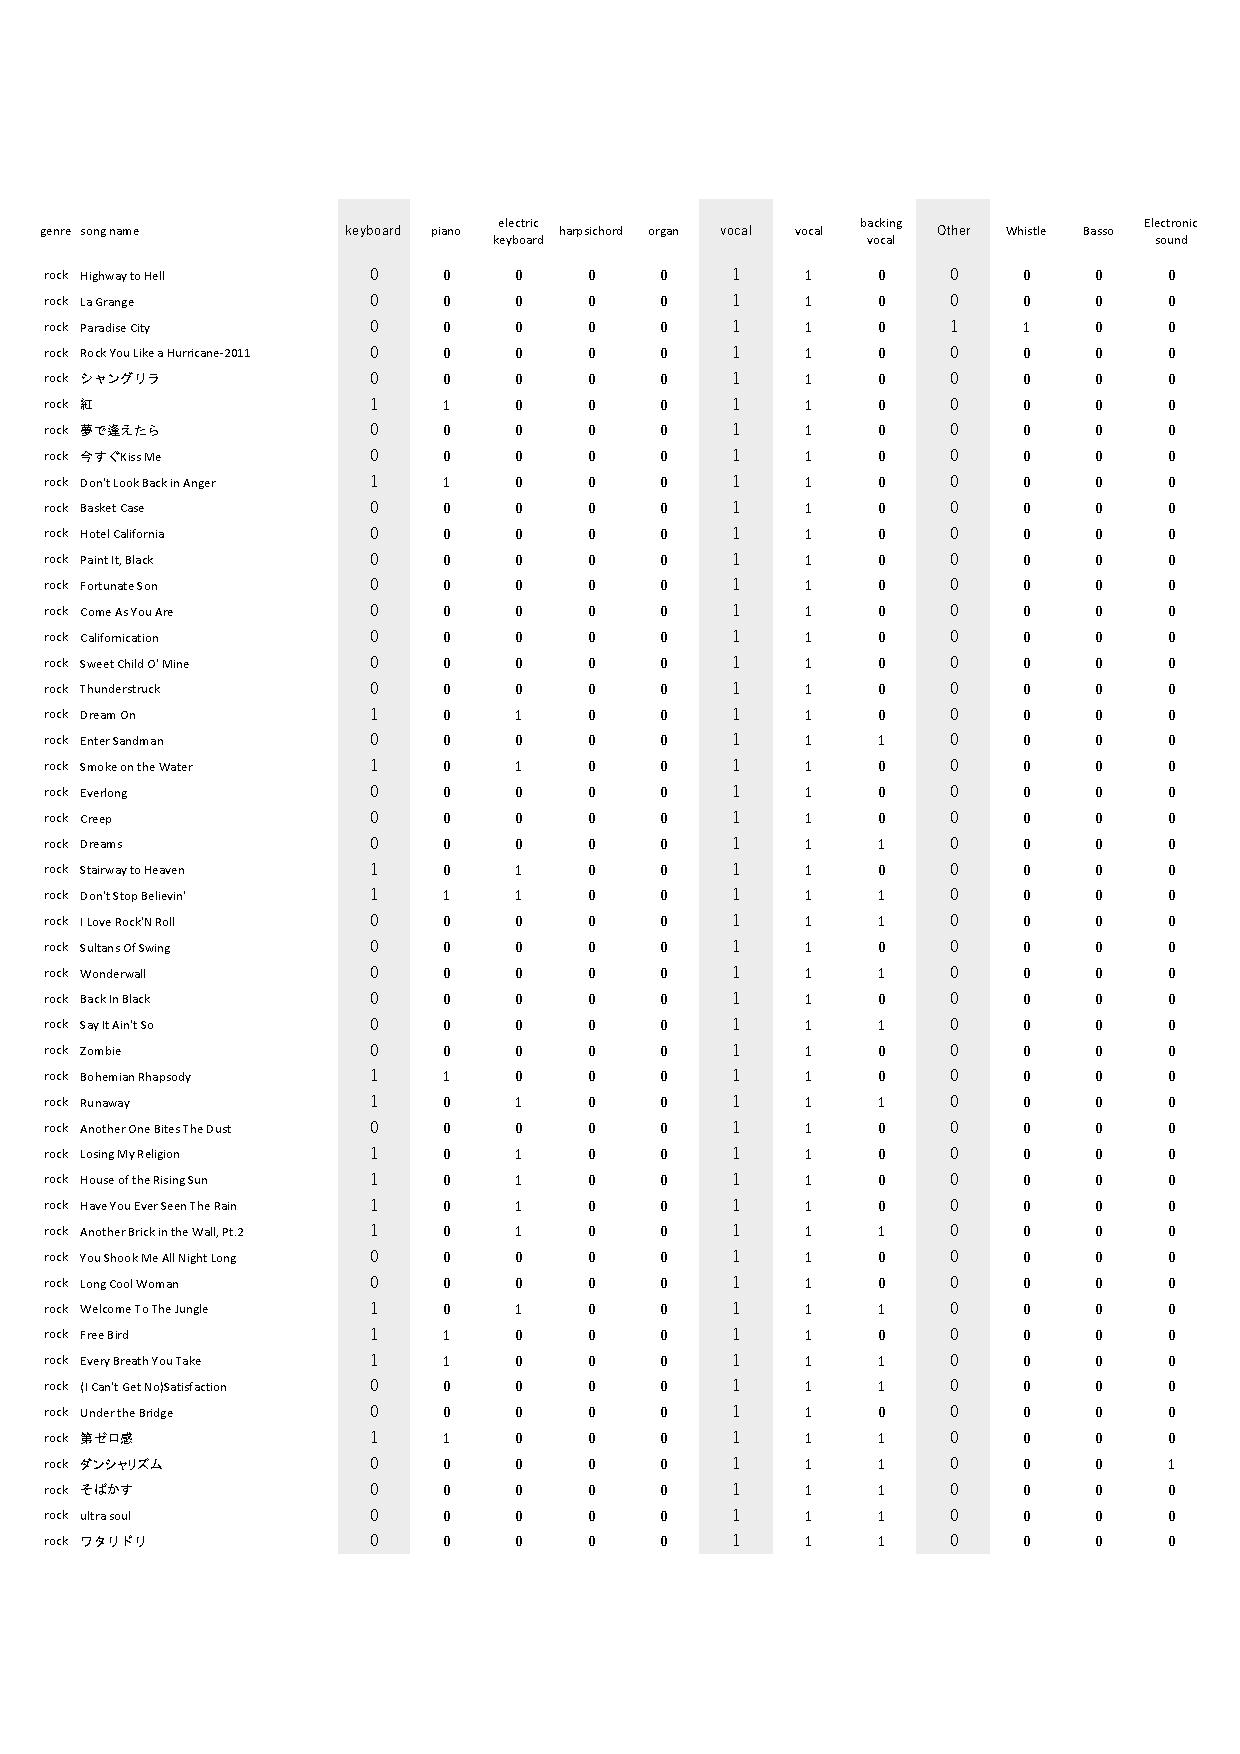
\includegraphics[width=.8\hsize]{fig/fig47-testdata11.pdf}
	\label{fig:11}
\end{figure*}

\begin{figure*}[tb]
	\centering
	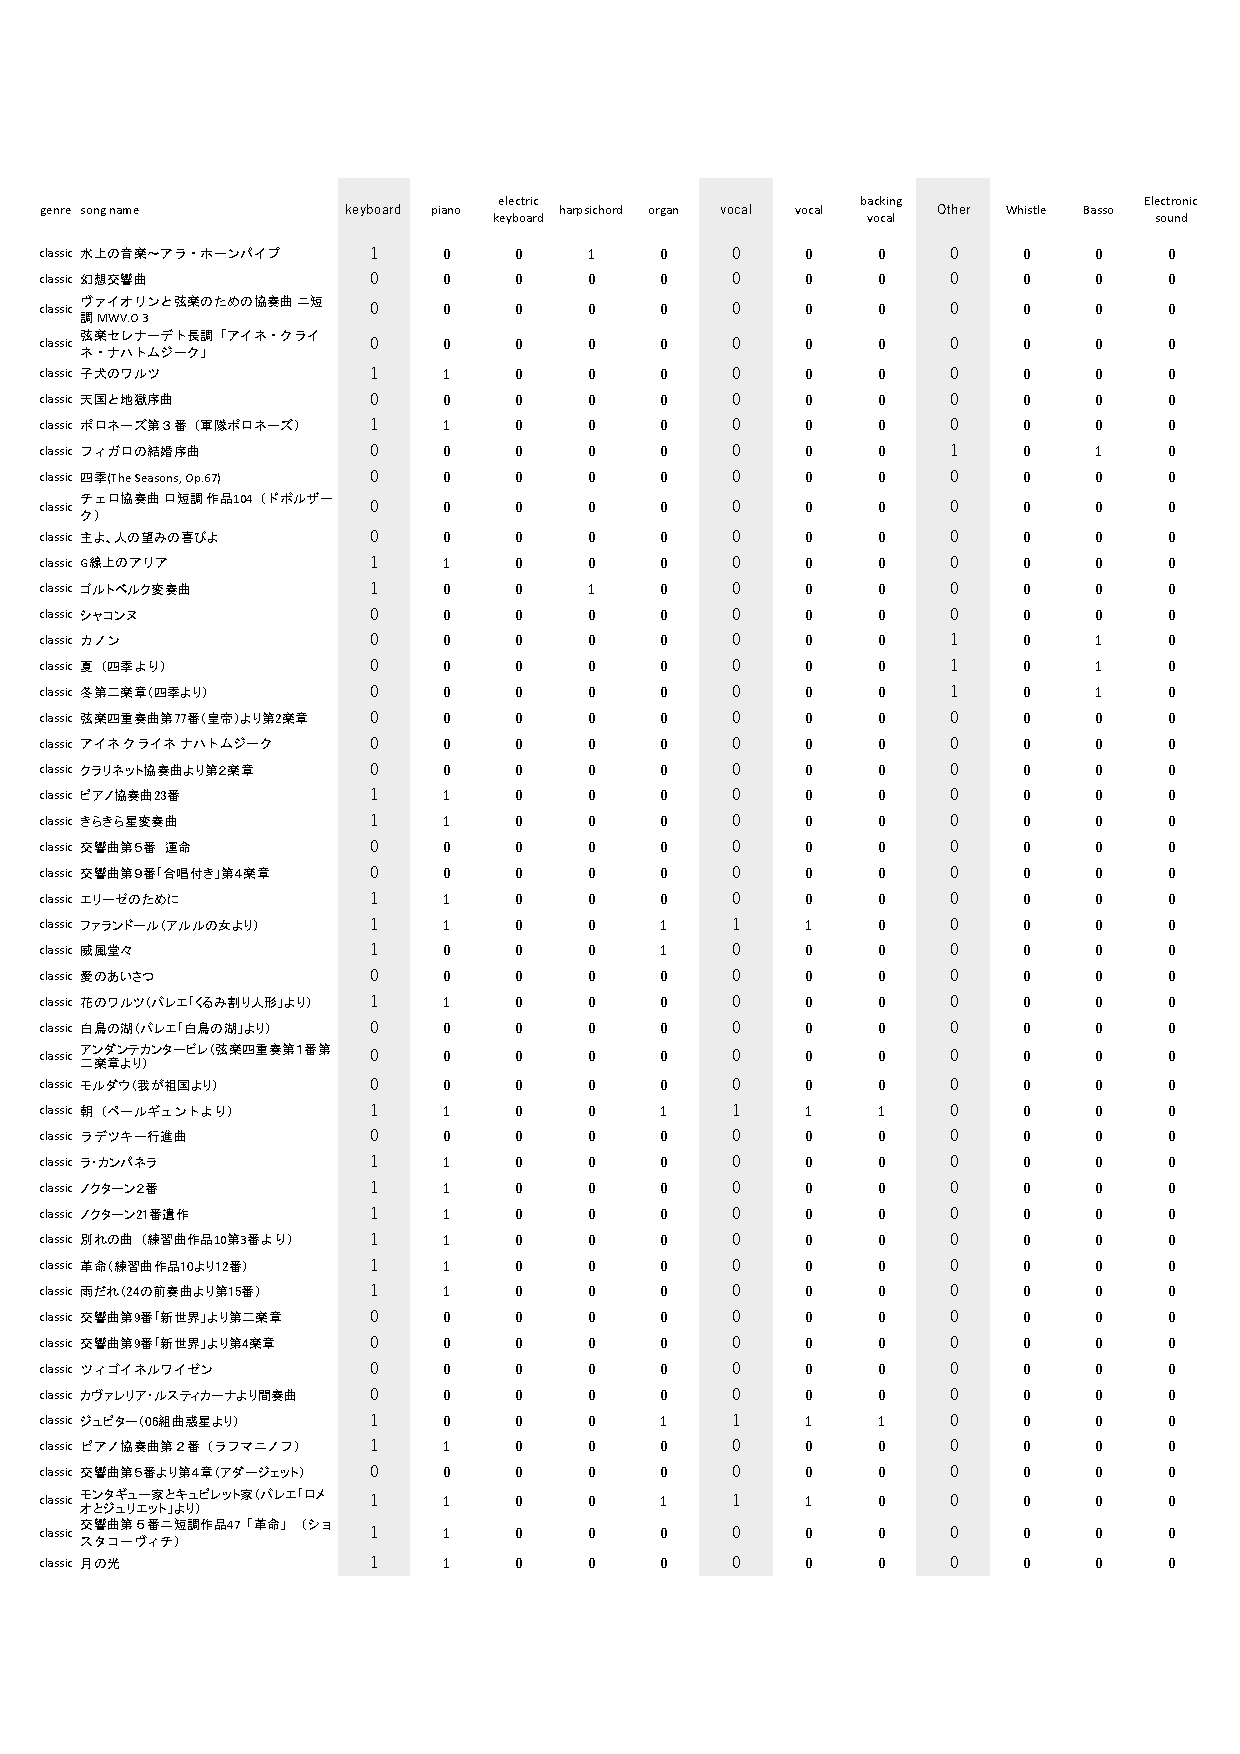
\includegraphics[width=.8\hsize]{fig/fig48-testdata12.pdf}
	\label{fig:12}
\end{figure*}

\begin{figure*}[tb]
	\centering
	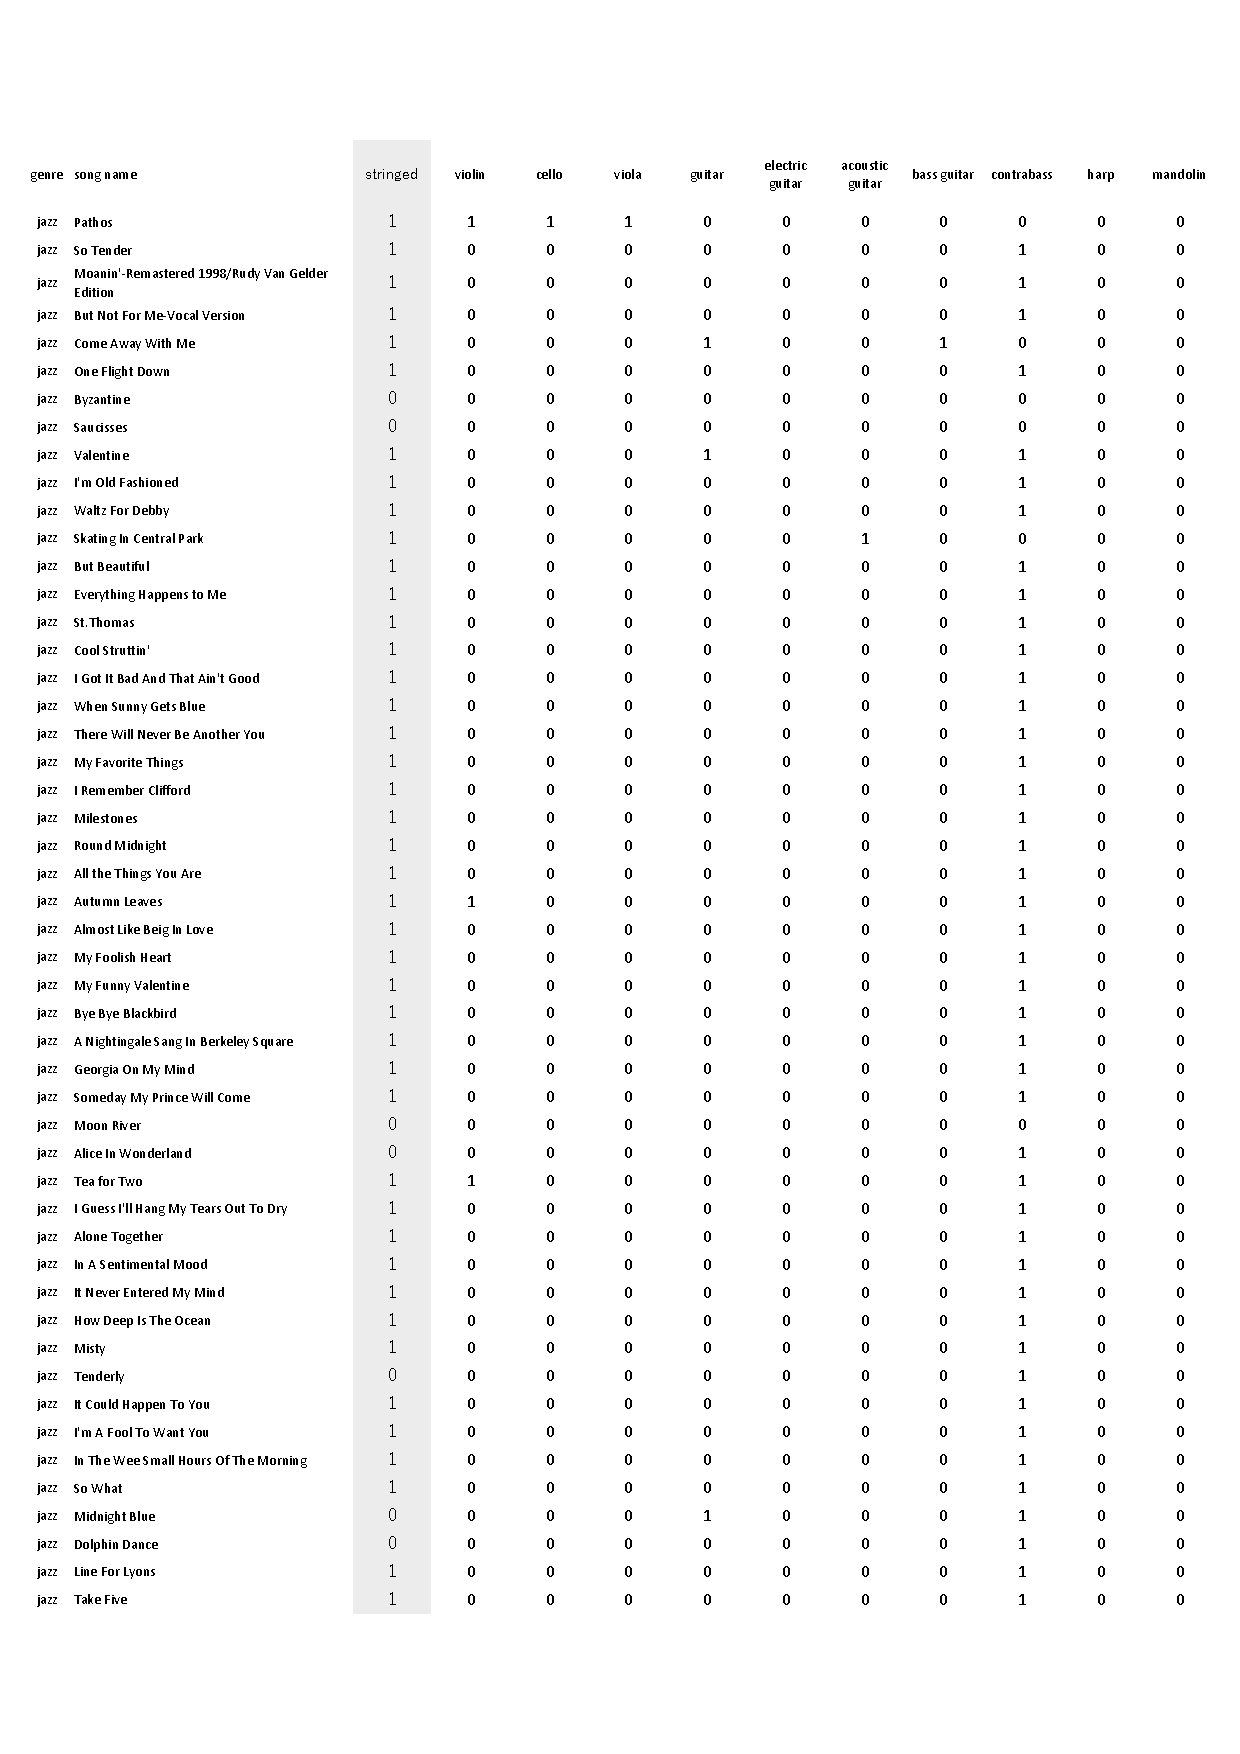
\includegraphics[width=.8\hsize]{fig/fig49-testdata13.pdf}
	\label{fig:13}
\end{figure*}

\begin{figure*}[tb]
	\centering
	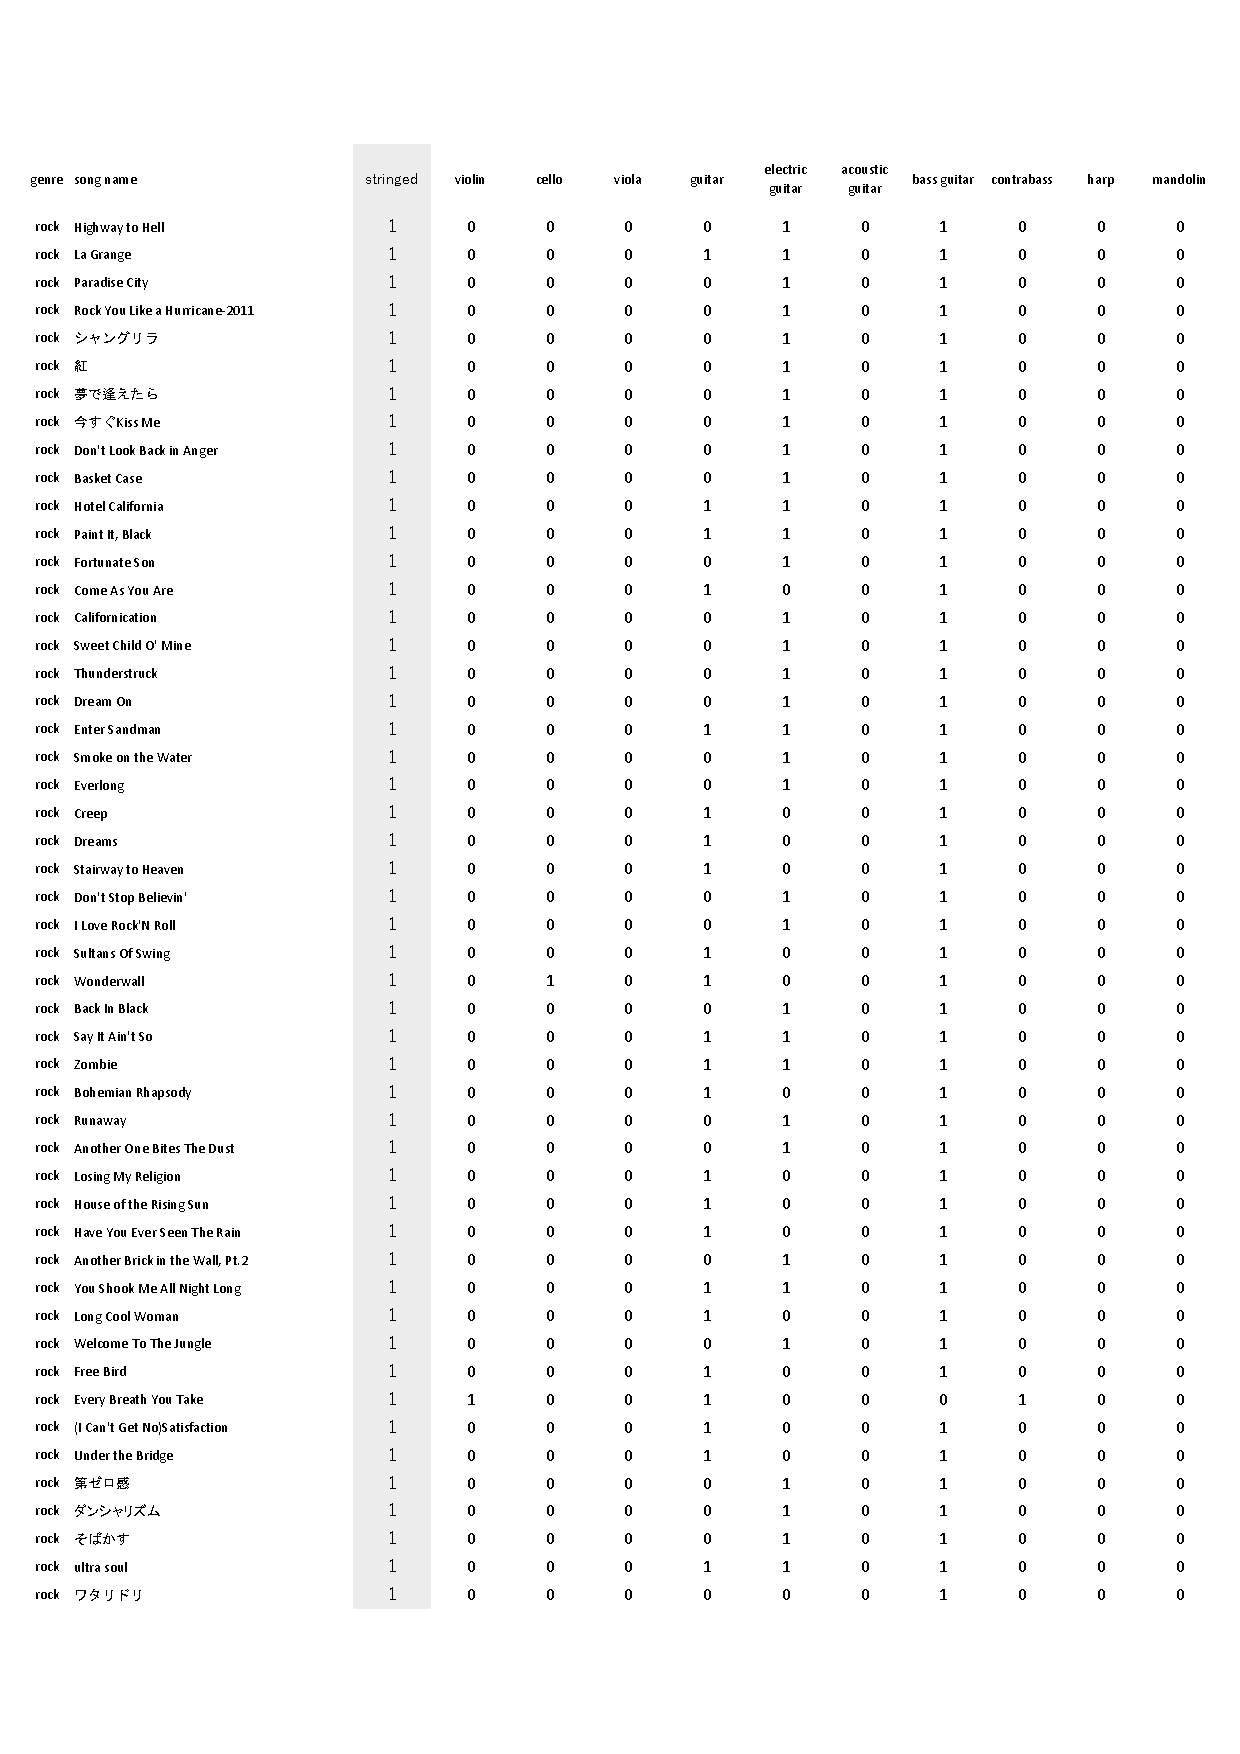
\includegraphics[width=.8\hsize]{fig/fig50-testdata14.pdf}
	\label{fig:14}
\end{figure*}

\begin{figure*}[tb]
	\centering
	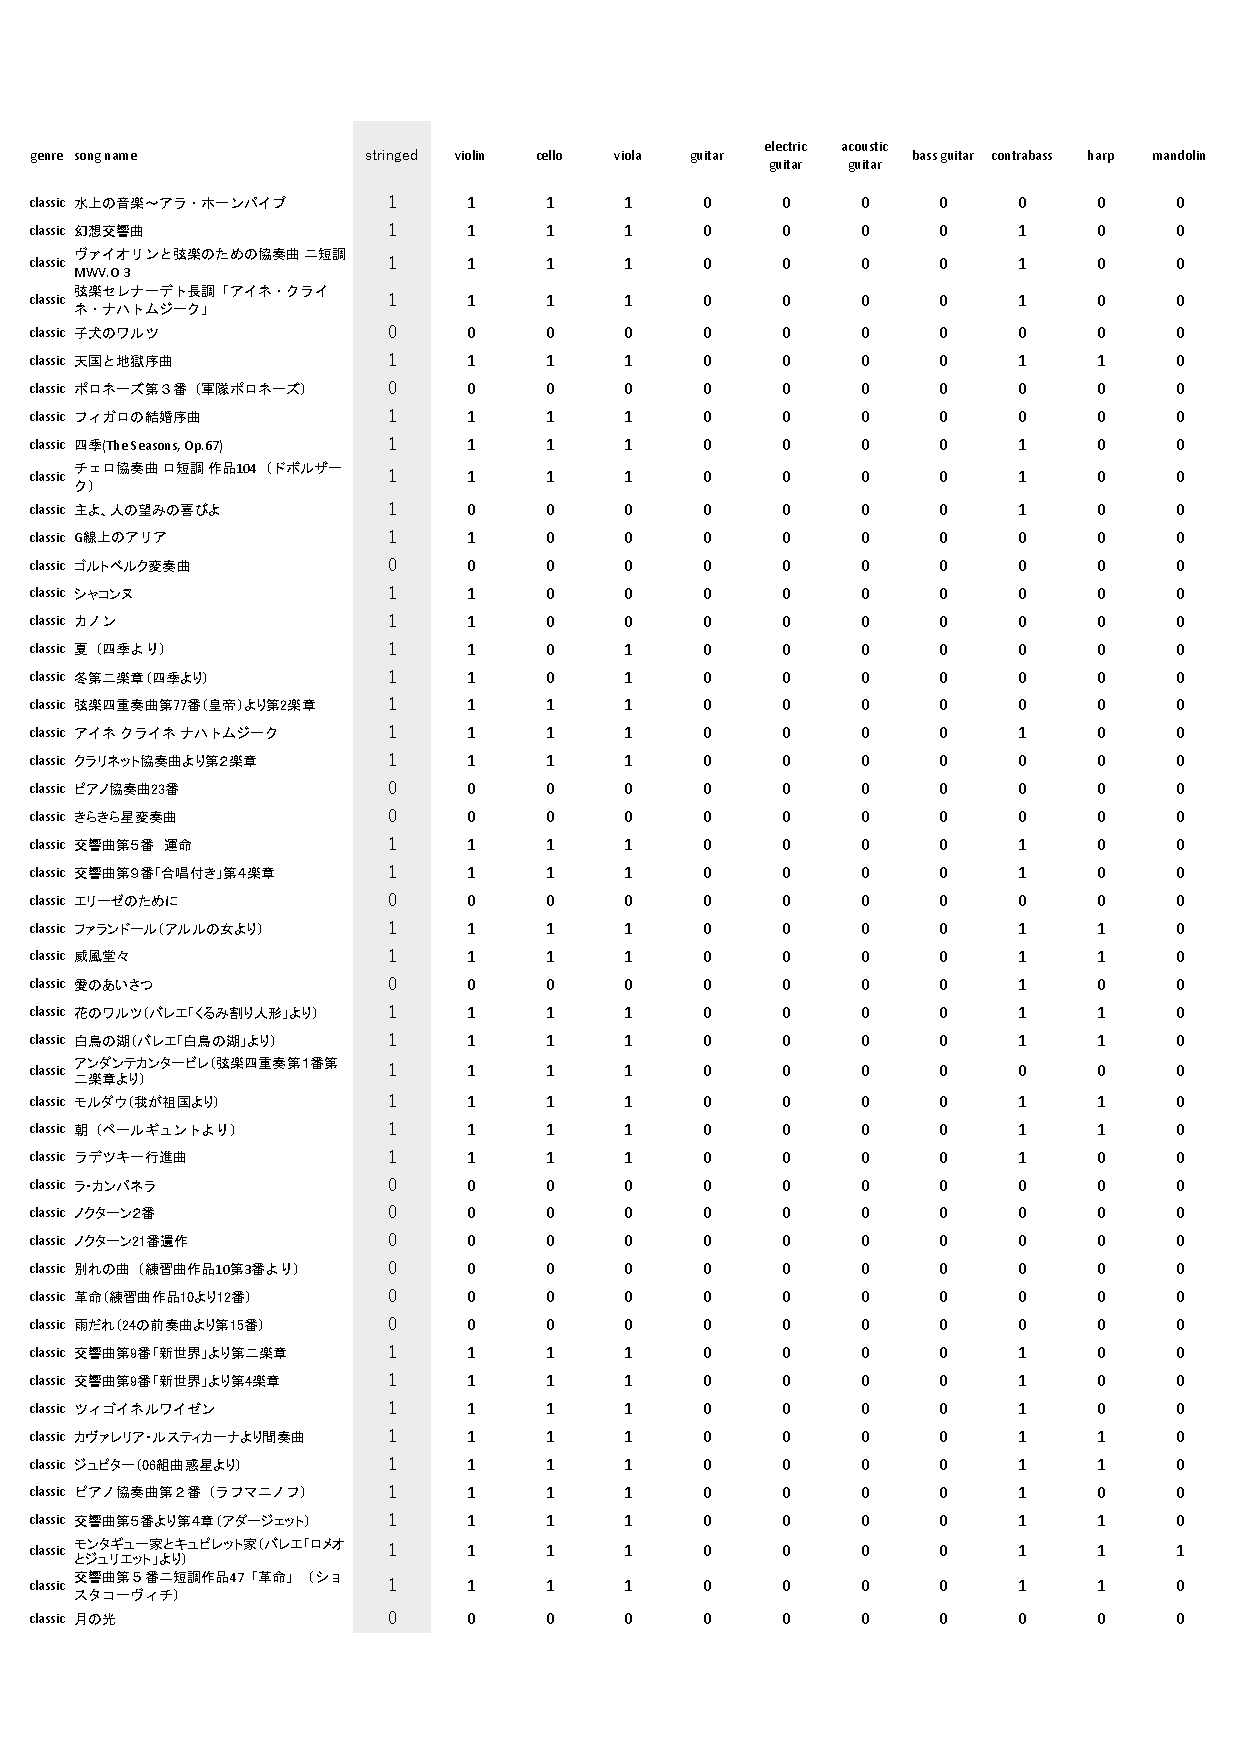
\includegraphics[width=.8\hsize]{fig/fig51-testdata15.pdf}
	\label{fig:15}
\end{figure*}